\chapter{Implementação}\label{cap_implementacao}

%\resumodocapitulo{Resumo opcional}

\section{Caminho de Dados}
{
    O caminho de dados projetado para a implementação da microarquitetura
    uniciclo é apresentado na Figura~\ref{fig:datapath}.
}

\begin{figure}[H]
\centering
    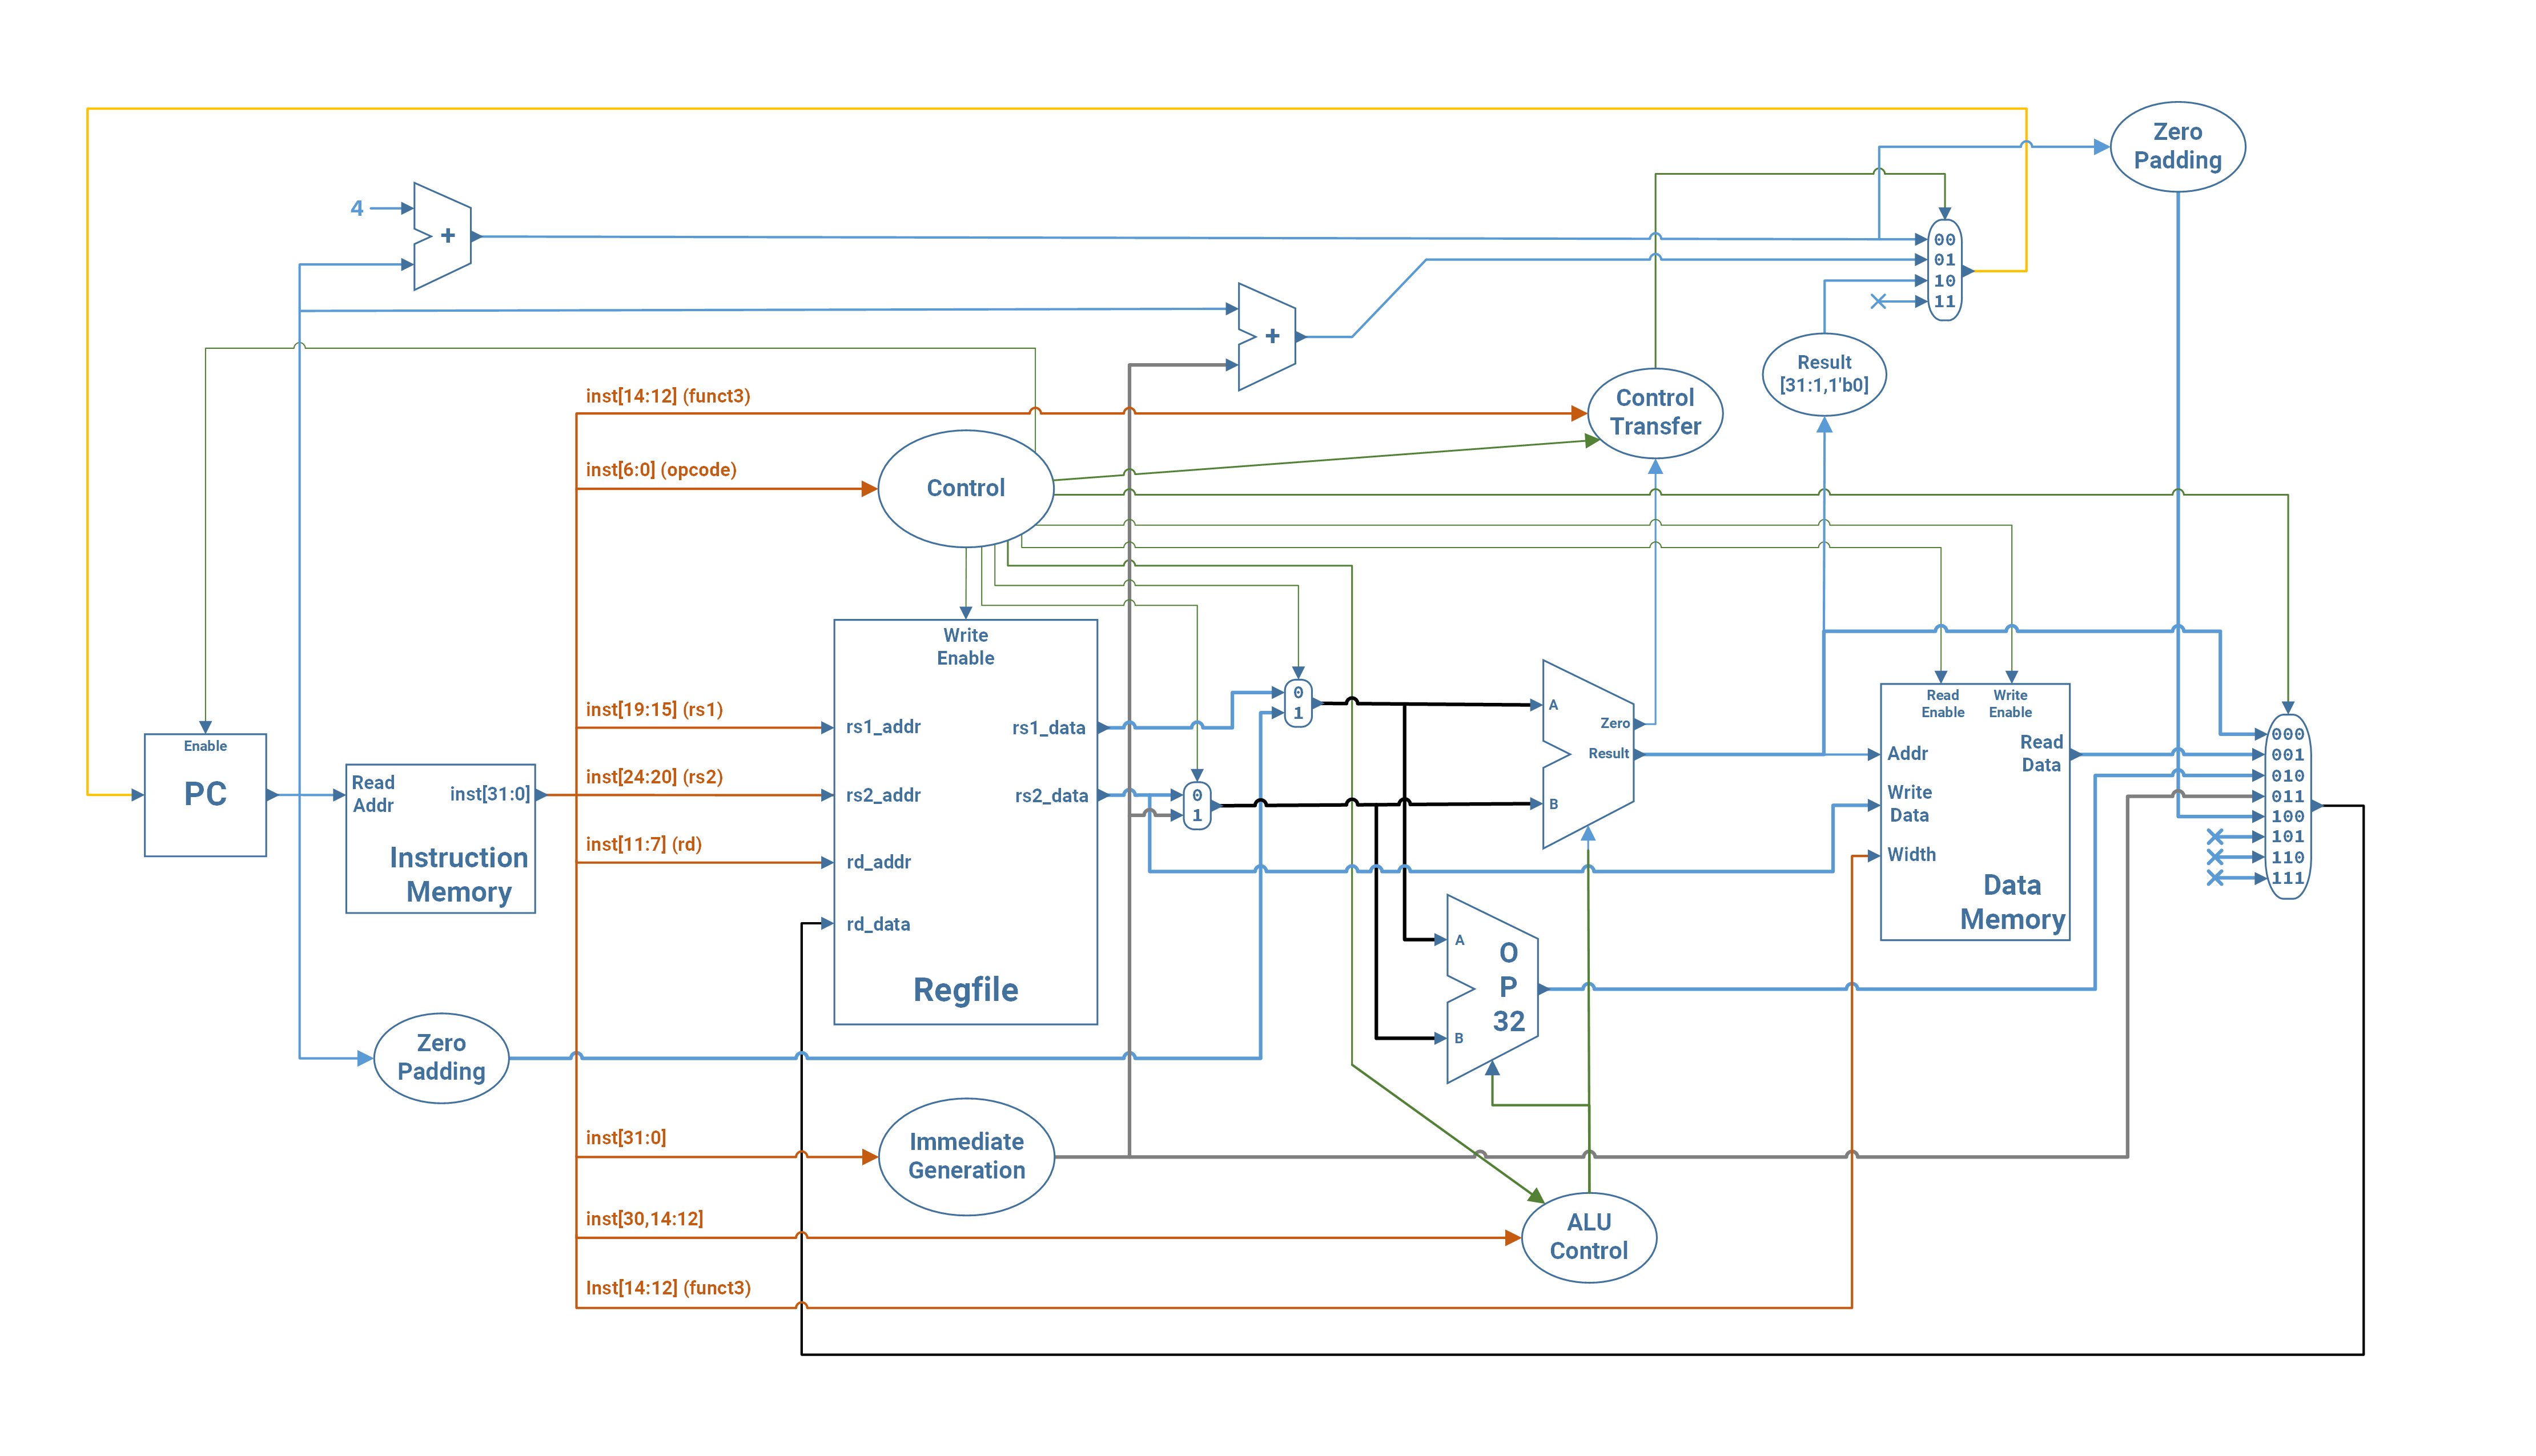
\includegraphics[width=1\linewidth]{../images/singlecycle.png}
    \caption{Caminho de Dados implementado para o
                módulo I}\label{fig:datapath}
\end{figure}

{
    O \textit{datapath} possui um banco de 32 registradores de uso geral
    de 64 bits cada. A memória possui arquitetura Harvard, sendo a memória
    de instruções (\textit{text}) \textit{read-only} e a memória de dados
    (\textit{data}) \textit{read-write}.
    São implementadas 49 instruções, sendo elas:
}

\begin{itemize}[leftmargin=20mm]
    \item {LUI:\@ Load Upper Intermediate;}
    \item {AUIPC:\@ Add Upper Intermediate to Program Counter;}
    \item {JAL:\@ Jump And Link;}
    \item {JALR:\@ Jump And Link Register;}
    \item {BEQ:\@ Branch if EQual;}
    \item {BNE:\@ Branch if Not Equal;}
    \item {BLT:\@ Branch if Less Than;}
    \item {BGE:\@ Branch if Greater or Equal;}
    \item {BLTU:\@ Branch if Less Than Unsigned;}
    \item {BGEU:\@ Branch if Greater or Equal Unsigned;}
    \item {LB:\@ Load Byte;}
    \item {LH:\@ Load Halfword;}
    \item {LW:\@ Load Word;}
    \item {LBU:\@ Load Byte Unsigned;}
    \item {LHU:\@ Load Halfword Unsigned;}
    \item {SB:\@ Store Byte;}
    \item {SH:\@ Store Halfword;}
    \item {SW:\@ Store Word;}
    \item {ADDI:\@ ADD Immediate;}
    \item {SLTI:\@ Set on Less Than;}
    \item {SLTIU:\@ Set on Less Than Unsigned;}
    \item {XORI:\@ XOR Immediate;}
    \item {ORI:\@ OR Immediate;}
    \item {ANDI:\@ AND Immediate;}
    \item {SLLI:\@ Shift Left Logical Immedate;}
    \item {SRLI:\@ Shift Right Logical Immediate;}
    \item {SRAI:\@ Shift Right Arithmetic Immediate;}
    \item {ADD:\@ ADD;}
    \item {SUB:\@ SUB;}
    \item {SLL:\@ Shift Left Logical;}
    \item {SLT:\@ Set on Less Than;}
    \item {SLTU:\@ Set on Less Than Unsigned;}
    \item {XOR:\@ XOR;}
    \item {SRL:\@ Shift Right Logical;}
    \item {SRA:\@ Shift Right Arithmetic;}
    \item {OR:\@ OR;}
    \item {AND:\@ AND;}
    \item {LWU:\@ Load Word Unsigned;}
    \item {LD:\@ Load Double;}
    \item {SD:\@ Store Double;}
    \item {ADDIW:\@ ADD Immediate Word-size;}
    \item {SLLIW:\@ Shift Left Logical Immedate Word-size;}
    \item {SRLIW:\@ Shift Right Logical Immediate Word-size;}
    \item {SRAIW:\@ Shift Right Arithmetic Immediate Word-size;}
    \item {ADDW:\@ ADD Word-size;}
    \item {SUBW:\@ SUB Word-size;}
    \item {SLLW:\@ Shift Left Logical Word-size;}
    \item {SRLW:\@ Shift Right Logical Word-size;}
    \item {SRAW:\@ Shift Right Arithmetic Word-size;}
\end{itemize}

{
    Para que o processador seja completamente compatível com a
    especificação da \textit{ISA}, falta implementar tratamentos de
    exceções, interrupções e \textit{traps}, Registradores \textit{CSR},
    instruções de chamada ao ambiente (ECALL/EBREAK), instruções de
    \textit{fencing} de memória, suporte ao acesso desalinhado à memória
    de dados e pilha de endereço de retorno (RAS).
}

